\begin{enumerate}
 \item D'après l'énoncé, on peut écrire des coordonnées :
 \begin{multline*}
  A:(a,0),\; B:(0,b),\; A'':(0,a),\; B':(b',0),\; \overrightarrow{A'A}:(a,-a'), \\
  \overrightarrow{B'B}:(-b',b).
 \end{multline*}
De plus $\overrightarrow{A'A}$ et $\overrightarrow{B'B}$ sont colinéaires au vecteur de coordonnées $(1,m)$ donc
\begin{displaymath}
 \left\lbrace
   \begin{align}
    -\frac{a'}{a} &= m \\ -\frac{b}{b'} &= m
   \end{align}
  \right. \Rightarrow
  \left\lbrace
  \begin{align}
   a' &= -ma \\ b' &= -\frac{b}{m}
  \end{align}
  \right. \Rightarrow
  M':(- \frac{b}{m}, -ma)
\end{displaymath}
Pour tout $(x,y)\in \R^2$, il existe un unique $(a,b)$ tel que $-\frac{b}{m} = x$  et $-ma = y$. C'est $a = - \frac{y}{m}$ et $b = -mx$. L'application $\mathcal{T}_m$ est donc bijective. Sa bijection réciproque est l'application qui à un point de coordonnées $(x,y)$ associe le point de coordonnées
\begin{displaymath}
 (-\frac{y}{m}, -mx).
\end{displaymath}
On en déduit $\mathcal{T}_m^{-1} = \mathcal{T}_m$.

 \item Soit $M$ de coordonnées $(a,b)$, remarquons que
\begin{displaymath}
 M = \mathcal{T}_m(M) \Leftrightarrow
 \left\lbrace
 \begin{align}
  -\frac{b}{m} &= a \\
  -ma &= b
 \end{align}
 \right. \Leftrightarrow b + am = 0.
\end{displaymath}
La droite $(M \mathcal{T}_m(M))$ est définie lorsque $b + am \neq 0$.\newline
Calculons les coordonnées
\begin{align*}
 \overrightarrow{M \mathcal{T}_m(P)} &: -\frac{b}{m} -a = -\frac{b+am}{m} &,&  -ma - b = - (b+am) \\
 P &: \frac{am - b}{2} &,& \frac{b-am}{2}.
\end{align*}
La direction de $(M \mathcal{T}_m(M))$ est $(1,m)$. Cette droite de pente $m$ est parallèle à $D_m$.\newline
Pour $m$ fixé, les milieux $P$ de $MM'$ décrivent la droite d'équation $x+y = 0$ c'est à dire la deuxième bissectrice des axes.\newline
Le fait que $P$ décrive la deuxième bissectrice fait penser que $\mathcal{T}$ pourrait être la symétrie orthogonale par  rapport à cette droite.\newline
Pour le vérifier, calculons les coordonnées $(x',y')$ du symétrique du point de coordonnées $(x,y)$. On a deux relations à vérifier: le milieu et l'orthogonalité.
\begin{displaymath}
 \left\lbrace
   \begin{aligned}
     \frac{x' + x}{2} + \frac{y' + y}{2} &= 0\\
     (x' - x) - (y' -y) &= 0
   \end{aligned}
 \right.  \Leftrightarrow
 \left\lbrace
   \begin{aligned}
     x' + y' &=  -x -y\\
     x' - y' &=  x - y
   \end{aligned}
 \right. \Leftrightarrow
 \left\lbrace
   \begin{aligned}
     x' &= -y \\ y' &= x
   \end{aligned}
 \right.
\end{displaymath}
Cette expression ne contient evidemment aucun $m$ donc $\mathcal{T}_m$ n'est pas cette symétrie orthogonale. Pourtant c'est bien une symétrie car $\mathcal{T}_m^{-1} = \mathcal{T}_m$. Il s'agit de la symétrie oblique par rapport à la deuxième directrice dans la direction $(1,m)$ daprès le calcul de $\overrightarrow{MM'}$.

\begin{figure}[!h]
 \centering
 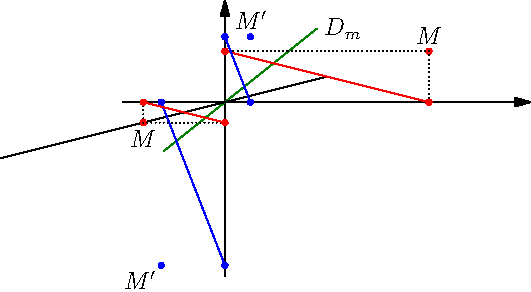
\includegraphics{Cgep1_1.pdf}
 \caption{3. Droites parallèles.}
\end{figure}

 \item
 \begin{enumerate}
  \item Fixons un point $M_0$ de coordonnées $(a,b)$ et. Alors les points $A$ et $B$ associés à ce $M_0$ sont respectivement de coordonnées $(a,0)$ et $(0,b)$. L'équation de la droite $(AB)$ est
  \begin{displaymath}
   \frac{x}{a} + \frac{x}{b} = 1.
  \end{displaymath}
  Considérons les autres points $M$ de la droite $(OM_0)$. Leurs coordonnées sont de la forme $(\lambda a, \lambda b)$ avec $\lambda$ réel. L'équation de la droite $(AB)$ associée est
  \begin{displaymath}
   \frac{x}{\lambda a} + \frac{x}{\lambda b} = 1 \Leftrightarrow \frac{x}{a} + \frac{x}{b} = \lambda.
  \end{displaymath}
  Ces droites sont donc parallèles entre elles.

  \item Les points $A'$ et $B'$ sont respectivement de coordonnées $(\frac{- \lambda b}{m},0)$ et $(0,-\lambda m a)$. L'équation de $(A',B)$ est
  \begin{displaymath}
   -\frac{m x}{\lambda b} - \frac{y}{\lambda m a} = 1 \Leftrightarrow \frac{m x}{b} + \frac{y}{ma} = \lambda .
  \end{displaymath}
Elles sont encore parallèles entre elles.
 \end{enumerate}

\begin{figure}[!h]
 \centering
 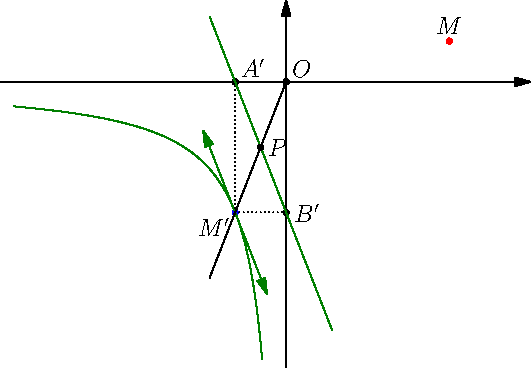
\includegraphics{Cgep1_2.pdf}
 \caption{4. Hyperbole.}
\end{figure}

 \item
 \begin{enumerate}
  \item Cette fois $M :(a,b)$ est fixé et $m>0$. Dans la rédaction de cette question, on confond un point avec son couple de coordonnées. L'ensemble $\mathcal{H}$ est l'image de la courbe paramétrée
  \begin{displaymath}
  h:
  \left\lbrace
   \begin{aligned}
    \left] 0, +\infty \right[ &\rightarrow \R^2 \\
    m &\rightarrow \left( -\frac{b}{m}, - ma \right)
   \end{aligned}
   \right.
  \end{displaymath}
  C'est une hyperbole d'équation $xy = ab$.

  \item On suppose que $M$ n'est pas sur les axes c'est à dire que $a$ et $b$ sont non nuls.\newline
  Le vecteur directeur de la tangente en $M'$ à l'hyperbole est la vitesse (dérivée).
  \begin{displaymath}
   h'(m) = \left( \frac{b}{m^2}, -a\right) \Rightarrow
  \end{displaymath}
  Le vecteur directeur de $(A',B')$ est
  \begin{displaymath}
   \overrightarrow{A'B'} = (-ma, \frac{b}{m}) \Rightarrow h'(m) = m \overrightarrow{A'B}.
  \end{displaymath}
  On en déduit que les droites sont parallèles donc homothétiques. Pour calculer le rapport de l'homothétie qui envoie $(A',B')$ sur la tangente , on forme le point d'intersection $P$ de $(OM')$ avec $(A'B')$. Le rapport cherché est le réel $\mu$ tel que
  \begin{displaymath}
   \overrightarrow{OM'} = \mu \overrightarrow{OP}.
  \end{displaymath}
  Les coordonnées de $P$ sont de la forme
  \begin{displaymath}
   \left( -\lambda \frac{b}{m}, - \lambda a m \right) \text{ avec } \lambda = \frac{1}{\mu} \text{ et } P, A', B' \text{ alignés.}
  \end{displaymath}
  On traduit l'alignement avec un déterminant
  \begin{displaymath}
   \begin{vmatrix}
    -\lambda \frac{b}{m} & - \lambda a m & 1 \\
    -\frac{b}{m}         & 0             & 1 \\
    0                    & -am           & 1
   \end{vmatrix}
   =0
   \Leftrightarrow
   ab - \lambda ab - \lambda ab = 0
   \Leftrightarrow \lambda = \frac{1}{2} \Leftrightarrow \mu = 2.
  \end{displaymath}
  en développant selon la dernière colonne.
 \end{enumerate}

\end{enumerate}
